\documentclass[a4paper,twoside, onecolumn]{IEEEtran}
\title{Bachelor thesis by Tim Budweg} 
\author{}
\date{11.03.2015}

\usepackage{graphicx}
\graphicspath{{figures/eps/}}

\newtheorem{emptycircle}{Lemma}[section]
\newtheorem{emptyregion}{Lemma}[section]
\begin{document}
\maketitle

\section{Introduction}
Wireless ad-hoc sensor networks are very useful. 
You can create warning systems for emergency purposes.
For instance, deploying many sensor nodes into the sea or forest to check and caution for tsunamis or fire.
Another use case is
\section{Algorithm}
\section{Reactive construction}
\section{Proof}
The authors of \cite{kanj} use $LDel^{(2)}(U) $ as the underlying subgraph of the Modified Yao Step.
$LDel^{(2)}(U) $ is defined as the subgraph of U in which the circumcircle of every triangle does not contain a 2-hop-neighbor of the nodes which create the triangle.
However, it is not known whether $LDel^{(2)}(U) $ can be constructed reactively.
At this point I want to introduce the Partial Delaunay Triangulation (PDT) \cite(pdt) which might be a valid replacement.


This proof is adapted from \cite{kanj}.
In a style similar to the proof from \cite{kanj}, we define the Partial Delaunay Triangulation (PTD) as follows:
\begin{emptycircle}
\label{emptycircle}
An edge XY of U is in the PDT graph if and only if there exists a circle trough X and Y whose interior contains no point of U that is a 2-hop neighbor of X or Y.
\end{emptycircle}
We need to show that the inward and outward path are still valid for PDT.
To do so, we must proof several properties, which are shown in figure $\cdots $

\begin{emptyregion}
If CA and CB are edges of G then the region of $(O)=\bigcirc{ABC} $ subtended by chord  CA and away from B and the region of $(O) $ subtended by chord CB and away from A contain no points that are two hop neighbors of A, B and C.
\end{emptyregion}

The edge CA is only contained in the graph G if there is a circle through C and A which contains no points of G.
The region of the circle $\bigcirc{ABC} $ subtended by chord CA and away from B is always contained completely in the circle through C and A.
Therefore, it must be empty, too.
For an illustration of this lemma have a look at figure \ref{fig:region}.


\begin{figure}[h!]
\centering
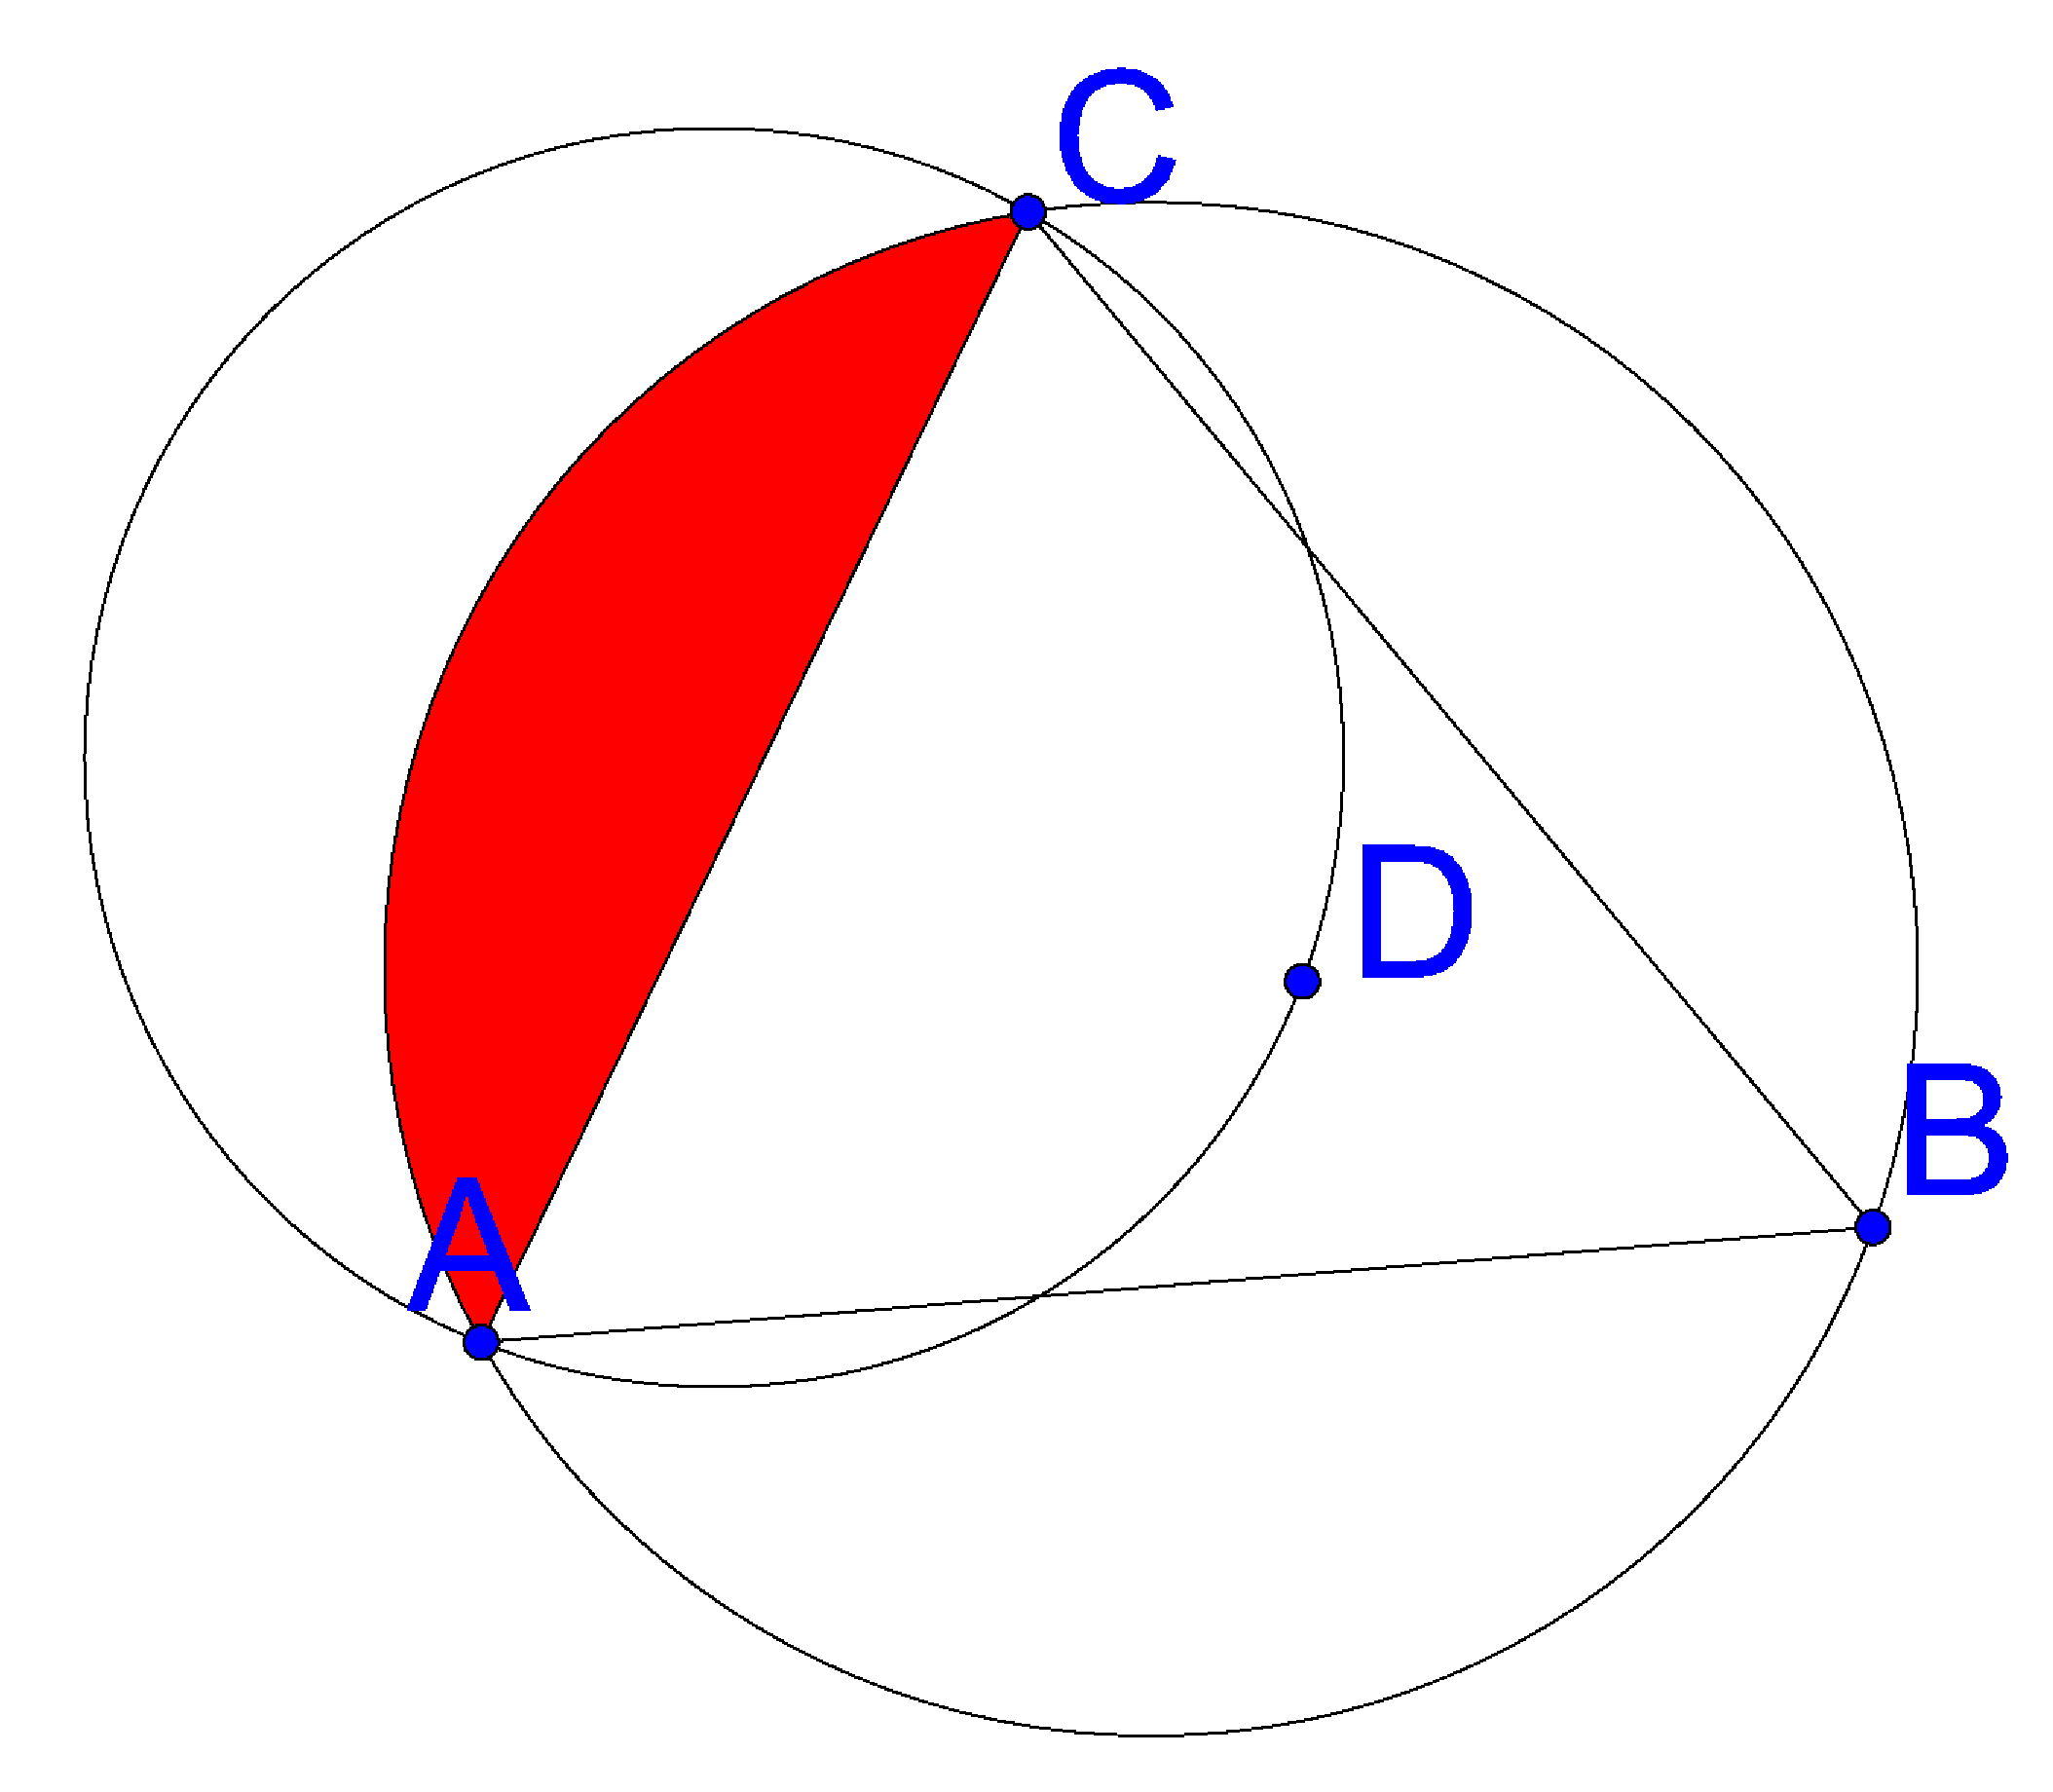
\includegraphics[width=0.2\linewidth]{noPointinRegion.eps}
\caption{The red marked region contains no Points of G because it is contained in $\bigcirc{ACD} $ which must be empty by definition.}
\label{fig:region}
\end{figure}

\section{Diskussion and Conclusion}

\section{Programming}

\bibliographystyle{IEEEtran}
\bibliography{biblio}
\end{document}